\subsection{Verifica}
\subsubsection{Scopo}
Lo scopo di questa sezione è definire come il gruppo ha deciso di attuare il processo di \glo{verifica}. Questo accerta che non siano stati introdotti errori durante lo sviluppo. Essa è svolta ripetutamente su tutti i processi in esecuzione (a ogni incremento della \glo{baseline}).

\subsubsection{Aspettative}
\begin{itemize}
	\item Verificare ogni fase rispettando criteri precisi, consistenti e modificabili se necessario;
	\item Automatizzare il più possibile le attività del processo;
	\item Rispettare gli obiettivi di copertura indicati nel \PdQ{};
	\item Verificare correttamente per ottenere successo in fase di validazione.
\end{itemize}

\subsubsection{Descrizione}
Il processo di verifica prevede due attività principali, svolte dai \glo{verificatori}:
\begin{itemize}
	\item \textbf{Analisi statica}: non richiede l'esecuzione dell'oggetto di verifica. Per questo motivo è applicabile ad ogni prodotto, accertando la conformità agli standard e convenzioni di stile;
	\item \textbf{Analisi dinamica}: richiede l'esecuzione dell'oggetto di verifica. Per questo motivo è applicabile al codice sviluppato ma non ai documenti. Accerta, tramite test, il funzionamento di ogni unità del codice presa singolarmente ma anche dell'intero sistema nella sua complessità.
\end{itemize}
\subsubsection{Istanziazione del processo}
\paragraph{Verifica della documentazione}
Il processo di verifica della documentazione consiste in un'analisi statica attraverso strumenti automatici o condotta a mano (\glo{desk check}) con, in questo caso, due possibili metodi di lettura:   

\renewcommand{\arraystretch}{1.5}
\renewcommand\extrarowheight{1.5pt}
\begin{longtable}{C{3cm} | C{4cm} C{3cm} C{5cm}}
		\rowcolor{coloreRosso}
		\textcolor{white}{\textbf{Metodo}} & 
		\textcolor{white}{\textbf{Obiettivo}} & 
		\textcolor{white}{\textbf{Attori}} & 
		\textcolor{white}{\textbf{Caratteristica}} \\
		\endfirsthead
		\rowcolor{white}\multicolumn{3}{C{8cm}}{\textit{Continua nella pagina successiva...}}\\
	    \endfoot
	    \rowcolor{white}\caption{Metodi di lettura}
	    \endlastfoot
		\hline
		\textbf{Walkthrough} & 
		Rilevare errori attraverso letture ad ampio spettro. & 
		Verificatori \newline Redattori & 
		Un errore riscontrato dal verificatore comporta una discussione con il redattore "colpevole" riguardo a una possibile soluzione. \\
		\textbf{Inspection} & 
		Rilevare specifici errori attraverso letture mirate. & 
		Verificatori \newline Redattori & 
		Il verificatore utilizza una lista di controllo, ossia un elenco di cosa va verificato in modo selettivo. \\
\end{longtable}


\textbf{Procedimento di verifica della documentazione}

Si riporta di seguito sotto forma di diagramma delle attività la procedura impiegata dal gruppo \Gruppo{} per la verifica dei documenti.


\begin{figure}[!htb]
   %\begin{minipage}{0.6\textwidth}
     \centering
     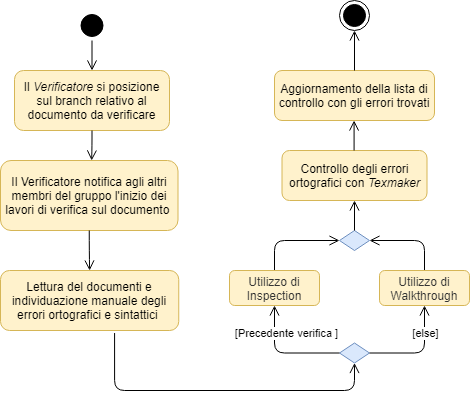
\includegraphics[scale=0.7]{Images/verDocs.png}
     \caption{Diagramma delle attività di verifica del codice}
   %\end{minipage}
\end{figure}



\paragraph{Verifica del codice}
Il processo di verifica del codice rappresenta l'unione delle attività di analisi statica e dinamica. 

\renewcommand{\arraystretch}{1.5}
\renewcommand\extrarowheight{1.5pt}
\begin{longtable}{C{3cm} | C{4cm} C{3cm} C{5cm}}
		\rowcolor{coloreRosso}
		\textcolor{white}{\textbf{Analisi}} & 
		\textcolor{white}{\textbf{Obiettivo}} & 
		\textcolor{white}{\textbf{Attori}} & 
		\textcolor{white}{\textbf{Esempi}} \\
		\endfirsthead
		\rowcolor{white}\multicolumn{3}{C{8cm}}{\textit{Continua nella pagina successiva...}}\\
	    \endfoot
	    \rowcolor{white}\caption{Analisi del codice}
	    \endlastfoot
		\hline
		\textbf{Statica} & 
		Verificare che siano rispettati i principi di buona programmazione preimpostati dal gruppo. & 
		Verificatori \newline Programmatori & 
		Analisi di flusso dei dati, verifica formale del codice ecc. \\
		\textbf{Dinamica} & 
		Trovare \glo{bug} ed errori eseguendo il prodotto software.  & 
		Verificatori \newline Programmatori & 
		Test di unità, di integrazione, di sistema, di regressione, di accettazione. \\
\end{longtable}

\textbf{Procedimento di verifica del codice}

Si riporta di seguito sotto forma di diagramma delle attività la procedura impiegata dal gruppo \Gruppo{} per la verifica del codice.


\begin{figure}[!htb]
   %\begin{minipage}{0.6\textwidth}
     \centering
     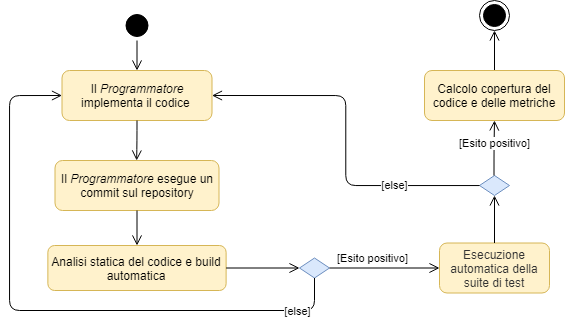
\includegraphics[scale=0.7]{Images/verCode.png}
     \caption{Diagramma delle attività di verifica della documentazione}
   %\end{minipage}
\end{figure}


\textbf{Principi di buona programmazione}\\
Il gruppo si pone come obiettivo quello di scrivere codice facilmente verificabile, favorendo il parallelismo tra i processi di sviluppo e verifica. I principi da rispettare sono:
\begin{itemize}
	\item Riflettere nel codice il \glo{design} progettato, utilizzando una programmazione strutturata;
	\item Separare le interfacce dalla loro implementazione (interfacce esposte, implementazioni nascoste);
	\item Massimizzare l'incapsulamento (\glo{information hiding});
	\item Usare tipi specializzati per specificare dati, aumentando il potere espressivo del sistema. 
\end{itemize}

\mbox{}

\textbf{Analisi di flusso dei dati} \\
Il gruppo effettua un'analisi statica del codice accertando che il programma in verifica non acceda in nessuna sua parte a variabili prive di valore, quindi non ancora scritte. Controlla l'assenza di dati globali.\\

\mbox{}

\textbf{Verifica formale} \\
Il gruppo effettua un'analisi statica del codice che ne prova la sua correttezza rispetto ai requisiti imposti dalle specifiche. Lo scopo è quello di esplorare tutti i rami possibili di esecuzione, senza doverlo necessariamente eseguire. \\

\mbox{}

\textbf{Test} \\
Questa attività ha lo scopo di rivelare al programmatore errori o \glo{bug} riscontrabili a run-time.
L'esecuzione dei test deve essere ripetibile ed è quindi buona pratica renderla il più possibile automatica. \\
Le specifiche dei test vengono elencate in forma tabellare, indicando per ciascuno: 
\begin{itemize}
	\item Il codice identificativo del test;
	\item La descrizione del test;
	\item Lo stato del test:
	\begin{itemize}
		\item \textbf{I}: Il test è stato implementato;
		\item \textbf{NI}: Il test non è stato implementato;
		\item \textbf{S}: Il test è passato con successo;
		\item \textbf{F}: Il test è fallito.
	\end{itemize}
\end{itemize}

\mbox{}

\textbf{Classificazione dei test} \\
I test sono identificati tramite un codice formato dai seguenti campi:
\begin{center}
\textbf{T[TipologiaTest][ImportanzaRequisito]*[TipologiaRequisito]*[IdNumerico]} 
\end{center}
Singolarmente essi rappresentano:
\begin{itemize}
	\item \textbf{TipologiaTest}: identifica la tipologia di test. Nello specifico:
		\begin{itemize}
			\item \textbf{U} : unità;
			\item \textbf{I} : integrazione;
			\item \textbf{S} : sistema;
			\item \textbf{R} : regressione.	 
		\end{itemize}
	\item \textbf{ImportanzaRequisito \& TipologiaRequisito}: sono seguiti da '*' perché presenti solo nei codici per i test di sistema. Questi campi identificano il requisito che si vuole testare (o più requisiti con la stessa importanza e stessa tipologia), seguendo ciò che è riportato al paragrafo \ref{para:requisiti} sotto la voce "Struttura dei requisiti;
	\item \textbf{IdNumerico}: codice numerico crescente che parte da 1 e distingue i test dello stesso tipo (U, I, S, R).
\end{itemize}
 
\subsubsection{Metriche}
Alcuni parametri per comprendere la tabella seguente:
\begin{itemize}
	\item \textbf{Budget at Completion (BAC)}: numero intero, corrisponde al budget totale allocato inizialmente per il progetto;
	
	\item \textbf{Number of Changed (NoC)}: numero di requisiti cambiati;
	
	\item \textbf{Number of Deleted (NoD)}: numero di requisiti eliminati;
	
	\item \textbf{Number of Added (NoA)}: numero di requisiti aggiunti;
	
	\item \textbf{Total Number of Initial Requirement (TNIR)}: numero totale dei requisiti iniziali;
	
	\item \textbf{Number of Satisfied (NoS)}: numero totale di requisiti soddisfatti;
	
	\item \textbf{Total number of Requirement (TnR)}: numero totale di requisiti;
	
	\item \textbf{Line of Code Executed (LCE)}: linee di codice eseguite dagli algoritmi di test;
	
	\item \textbf{Line of Code(LC)}: linee di codice totali;
	
	\item \textbf{Number of Quality Metrics Satisfied (NQMS)}: numero di metriche di qualità soddisfatte;
	
	\item \textbf{Total number of Quality Metrics (TQM)}: numero totale di metriche di qualità;
	
	\item \textbf{Passed test cases percentage (PTCP)}: numero totale di metriche di qualità;
	
	\item \textbf{Failed test cases percentage (FTCP)}: numero totale di metriche di qualità.
	
\end{itemize}

\renewcommand{\arraystretch}{1.5}
\renewcommand\extrarowheight{1.5pt}
\begin{longtable}{C{1.5cm} C{4.5cm} C{5cm} C{4.5cm}}
		\rowcolor{coloreRosso}
		\textcolor{white}{\textbf{Codice}} & 
		\textcolor{white}{\textbf{Nome}} & 
		\textcolor{white}{\textbf{Descrizione}} & 
		\textcolor{white}{\textbf{Formula}} \\
		\endfirsthead
	    \endfoot
	    \rowcolor{white}\caption{Metriche per i processi}
	    \endlastfoot
		\hline
		\textbf{MPC1} & 
		Schedule Variance (SV)  & 
		Descrive se il gruppo sta rispettando o meno i tempi prestabiliti per i processi. & 
		((EV / PV) - 1) $\cdot 100$ \\
		
		\textbf{MPC2} & 
		Budget Variance (BV) & 
		Descrive se il gruppo sta rispettando o meno i costi prestabiliti per i processi. & 
		((EV / AC) - 1) $\cdot 100$ \\
		
		\textbf{MPC3} &
		Estimated at Completion (EAC) &
		Indica il budget totale allocato per il progetto. &
		AC + ETC \\
		
		\textbf{MPC4} &
		Earned Value (EV) &
		Rappresenta il valore prodotto dal progetto fino al momento della misurazione in seguito alle attività svolte.  &
		\% completamento $ \cdot EAC $\\
				
		\textbf{MPC5} &
		Planned Value (PV) &
		Corrisponde al denaro che si dovrebbe guadagnare al momento della misurazione.  &
		\% lavoro pianificato $ \cdot BAC $ \\
		
		\textbf{MPC6} &
		Actual Cost (AC) &
		soldi spesi per il progetto fino al momento del calcolo. &
		Numero intero \\
		
		\textbf{MPC7} &
		Estimate to Complete (ETC) &
		Valore stimato delle attività necessarie per il completamento del progetto.  &
		Numero intero \\	
			
		
		\textbf{MPC8} &
		Requirements stability index (RSI) &
		Indica quanto i requisiti variano nel tempo. &
		$(1 - \frac{NoC + NoD + NoA}{TNIR}) \cdot 100$ \\
		
		\textbf{MPC9} &
		Satisfied obligatory requirements (SOR) &
		Descrive se il gruppo ha soddisfatto i requisiti obbligatori o meno. &
		$\frac{NoS}{TnR} \cdot 100$ \\ 
		
		\textbf{MPC10} &
		Code Coverage (CC) &
		Descrive quanto il codice prodotto è coperto dalla suite di test dinamici. & $\frac{LCE}{LC}\cdot 100$ \\ 
		
		\textbf{MPC11} &
		Passed test cases percentage (PTCP) &
		Corrisponde alla percentuale di test passati rispetto alla suite di test dinamici. &
		Test passati / Test totali \\ 
		
		\textbf{MPC12} &
		Failed test cases percentage (FTCP) &
		Corrisponde alla percentuale di test falliti rispetto alla suite di test dinamici. &
		Test falliti / Test Totali \\ 
		
		\textbf{MPC13} &
		Quality Metrics Satisfied (QMS) &
		Descrive la percentuale di metriche di qualità soddisfatte. &
		$\frac{NQMS}{TQM} \cdot 100$ \\
		
		\textbf{MPC14} &
		Non-calculated Risk (NR) &
		Indica il numero di rischi non preventivati. &
		Numero intero 
\end{longtable}

\subsubsection{Strumenti}
Gli strumenti utilizzati in questo processo comprendono:
\begin{itemize}
	\item \textbf{Texmaker}: mette a disposizione un correttore automatico che individua le parole grammaticalmente scorrette sottolineandole in rosso;
	\item \textbf{Jest}: \glo{framework} di testing utilizzato per testare il codice \glo{JavaScript} e le attività interne delle componenti \glo{React};
	\begin{center}
		\textcolor{blue}{\url{https://jestjs.io/}}
	\end{center}
	\item \textbf{ESLint}: programma utilizzato per l'analisi statica del codice. Nello specifico, il tipo di analisi effettuata è chiamata \glo{code linting}. Questo programma mette a disposizione regole sintattiche che il codice deve rispettare e permette di definirne di nuove;
	\begin{center}
		\textcolor{blue}{\url{https://eslint.org/}}
	\end{center}
	\item \textbf{SonarCloud}: servizio web che permette di eseguire controlli del codice presente all'interno di un \glo{repository} e di riportare i risultati delle analisi in un cruscotto accessibile tramite web. Può quindi essere integrato con il \glo{repository} di \glo{GitHub} del gruppo, in modo che ad ogni caricamento o modifica il software analizzi il codice. Il cruscotto dei risultati è disponibile nel profilo del team e viene riportato come badge sul \glo{repository} stesso;
	\begin{center}
		\textcolor{blue}{\url{https://sonarcloud.io/}}
	\end{center}
	\item \textbf{Codecov}: strumento utilizzato per stabilire la percentuale di codice coperto dai test implementati. Questo strumento viene integrato nel \glo{repository} di \glo{GitHub} del gruppo tramite \glo{GitHub Action} e ad ogni \glo{build} i risultati vengono aggiornati nel profilo. La percentuale di \glo{code coverage} viene riportata come badge sul \glo{repository} stesso; 
	\begin{center}
		\textcolor{blue}{\url{https://sonarcloud.io/}}
	\end{center}
	\item \textbf{React Testing Library}: libreria utilizzata per testare e \glo{renderizzare} le componenti \glo{React} del prodotto.
	\begin{center}
		\textcolor{blue}{\url{https://testing-library.com/}}
	\end{center}	
\end{itemize}

